\documentclass[8pt]{article}
\RequirePackage{amsmath}
\RequirePackage{bytefield}
\RequirePackage{graphicx}
\RequirePackage{newtxmath}
\RequirePackage{mathtools}
\RequirePackage{xspace}
\RequirePackage{url}

\setlength{\oddsidemargin}{-0.25in} % Left margin of 1 in + 0 in = 1 in
\setlength{\textwidth}{7in}   % Right margin of 8.5 in - 1 in - 6.5 in = 1 in
\setlength{\topmargin}{-.75in}  % Top margin of 2 in -0.75 in = 1 in
\setlength{\textheight}{9.2in}  % Lower margin of 11 in - 9 in - 1 in = 1 in

\mathchardef\mhyphen="2D

% terminology

\newcommand{\term}[1]{\textsl{#1}\xspace}
\newcommand{\termbf}[1]{\textbf{#1}\xspace}

\newcommand{\Zcash}{\termbf{Zcash}}
\newcommand{\Zerocash}{\termbf{Zerocash}}
\newcommand{\Bitcoin}{\termbf{Bitcoin}}
\newcommand{\ZEC}{\termbf{ZEC}}
\newcommand{\zatoshi}{\term{zatoshi}}

\newcommand{\coin}{\term{coin}}
\newcommand{\coins}{\term{coins}}
\newcommand{\coinCommitment}{\term{coin commitment}}
\newcommand{\coinCommitments}{\term{coin commitments}}
\newcommand{\coinCommitmentTree}{\term{coin commitment tree}}
\newcommand{\PourDescription}{\term{Pour description}}
\newcommand{\PourDescriptions}{\term{Pour descriptions}}
\newcommand{\PourTransfer}{\term{Pour transfer}}
\newcommand{\PourTransfers}{\term{Pour transfers}}
\newcommand{\fullnode}{\term{full node}}
\newcommand{\fullnodes}{\term{full nodes}}
\newcommand{\anchor}{\term{anchor}}
\newcommand{\anchors}{\term{anchors}}
\newcommand{\block}{\term{block}}
\newcommand{\blocks}{\term{blocks}}
\newcommand{\transaction}{\term{transaction}}
\newcommand{\transactions}{\term{transactions}}
\newcommand{\blockchainview}{\term{blockchain view}}
\newcommand{\mempool}{\term{mempool}}
\newcommand{\treestate}{\term{treestate}}
\newcommand{\treestates}{\term{treestates}}
\newcommand{\script}{\term{script}}
\newcommand{\serialNumber}{\term{serial number}}
\newcommand{\serialNumbers}{\term{serial numbers}}
\newcommand{\publicAddress}{\term{confidential address}}
\newcommand{\privateAddress}{\term{confidential private key}}
\newcommand{\transmittedPlaintext}{\term{transmitted coin plaintext}}
\newcommand{\transmittedCiphertext}{\term{transmitted coin ciphertext}}
\newcommand{\transmitPublicAlgorithm}{\term{key-private encryption}}
\newcommand{\transmitPrivateAlgorithm}{\term{key-private decryption}}
\newcommand{\spendAuthority}{\term{spend authority}}
\newcommand{\incrementalMerkleTree}{\term{incremental merkle tree}}
\newcommand{\spentSerialsMap}{\term{spent serial numbers map}}
\newcommand{\zkSNARK}{\term{zk-SNARK}}
\newcommand{\zkSNARKs}{\term{zk-SNARKs}}

% key pairs:
\newcommand{\PublicAddress}{\mathsf{addr_{pk}}}
\newcommand{\PrivateAddress}{\mathsf{addr_{sk}}}
\newcommand{\PublicAddressLeadByte}{\mathbf{0x92}}
\newcommand{\PrivateAddressLeadByte}{\mathbf{0x93}}
\newcommand{\SpendAuthorityPublic}{\mathsf{a_{pk}}}
\newcommand{\SpendAuthorityPrivate}{\mathsf{a_{sk}}}
\newcommand{\SpendAuthorityPublicOld}[1]{\mathsf{a^{old}_{pk,\mathnormal{#1}}}}
\newcommand{\SpendAuthorityPrivateOld}[1]{\mathsf{a^{old}_{sk,\mathnormal{#1}}}}
\newcommand{\SpendAuthorityPublicNew}[1]{\mathsf{a^{new}_{pk,\mathnormal{#1}}}}
\newcommand{\SpendAuthorityPrivateNew}[1]{\mathsf{a^{new}_{sk,\mathnormal{#1}}}}
\newcommand{\TransmitPublic}{\mathsf{pk_{enc}}}
\newcommand{\TransmitPrivate}{\mathsf{sk_{enc}}}
\newcommand{\Value}{\mathsf{v}}

% Coins
\newcommand{\Coin}{\mathbf{c}}
\newcommand{\CoinCommitRand}{\mathsf{r}}
\newcommand{\CoinCommitRandOld}[1]{\mathsf{r^{old}_\mathnormal{#1}}}
\newcommand{\CoinCommitRandNew}[1]{\mathsf{r^{new}_\mathnormal{#1}}}
\newcommand{\CoinAddressRand}{\mathsf{\uprho}}
\newcommand{\CoinAddressRandOld}[1]{\mathsf{\uprho^{old}_\mathnormal{#1}}}
\newcommand{\CoinAddressRandNew}[1]{\mathsf{\uprho^{new}_\mathnormal{#1}}}
\newcommand{\TransmitPlaintextVersionByte}{\mathbf{0x00}}
\newcommand{\CRH}{\mathsf{CRH}}
\newcommand{\PRF}[2]{\mathsf{{PRF}^{#2}_\mathnormal{#1}}}
\newcommand{\PRFaddr}[1]{\PRF{#1}{addr}}
\newcommand{\PRFsn}[1]{\PRF{#1}{sn}}
\newcommand{\PRFpk}[2]{\PRF{#1}{pk,{\mathnormal{#2}}}}
\newcommand{\SHA}{\mathtt{SHA256Compress}}
\newcommand{\SHAName}{\term{SHA-256 compression}}
\newcommand{\SHAOrig}{\term{SHA-256}}
\newcommand{\cm}{\mathsf{cm}}
\newcommand{\cmNew}[1]{\mathsf{{cm}^{new}_\mathnormal{#1}}}
\newcommand{\InternalHashK}{\mathsf{k}}
\newcommand{\InternalHash}{\mathsf{InternalH}}

% merkle tree
\newcommand{\MerkleDepth}{\mathsf{d}}
\newcommand{\sn}{\mathsf{sn}}
\newcommand{\snOld}[1]{\mathsf{{sn}^{old}_\mathnormal{#1}}}

% bitcoin
\newcommand{\vin}{\mathtt{vin}}
\newcommand{\vout}{\mathtt{vout}}
\newcommand{\vpour}{\mathtt{vpour}}
\newcommand{\vpubOldField}{\mathtt{vpub\_old}}
\newcommand{\vpubNewField}{\mathtt{vpub\_new}}
\newcommand{\vsum}[2]{\smashoperator[r]{\sum_{#1}^{#2}}}
\newcommand{\anchorField}{\mathtt{anchor}}
\newcommand{\scriptSig}{\mathtt{scriptSig}}
\newcommand{\scriptPubKey}{\mathtt{scriptPubKey}}
\newcommand{\serials}{\mathtt{serials}}
\newcommand{\commitments}{\mathtt{commitments}}
\newcommand{\TransmitCiphertexts}{\mathtt{ciphertexts}}
\newcommand{\rt}{\mathsf{rt}}

% pour
\newcommand{\hSig}{\mathsf{h_{Sig}}}
\newcommand{\h}[1]{\mathsf{h_{\mathnormal{#1}}}}
\newcommand{\NOld}{\mathrm{N}^\mathsf{old}}
\newcommand{\NNew}{\mathrm{N}^\mathsf{new}}
\newcommand{\vmacs}{\mathtt{vmacs}}
\newcommand{\zkproof}{\mathtt{zkproof}}
\newcommand{\PourCircuit}{\term{\texttt{POUR} circuit}}
\newcommand{\PourStatement}{\texttt{POUR}}
\newcommand{\PourProof}{\pi_{\PourStatement}}
\newcommand{\vpubOld}{\mathsf{v_{pub}^{old}}}
\newcommand{\vpubNew}{\mathsf{v_{pub}^{new}}}
\newcommand{\cOld}[1]{\mathbf{c}_{#1}^\mathsf{old}}
\newcommand{\cNew}[1]{\mathbf{c}_{#1}^\mathsf{new}}
\newcommand{\vOld}[1]{\mathsf{v}_{#1}^\mathsf{old}}
\newcommand{\vNew}[1]{\mathsf{v}_{#1}^\mathsf{new}}
\newcommand{\NP}{\mathsf{NP}}
\newcommand{\treepath}[1]{\mathsf{path}_{#1}}
\newcommand{\COMM}[1]{\mathsf{COMM}_{#1}}
\newcommand{\COMMtrapdoor}{\term{\textsf{COMM} trapdoor}}
\newcommand{\CoinCommitment}[1]{\mathtt{CoinCommitment}(#1)}

\RequirePackage[usenames,dvipsnames]{xcolor}
% https://en.wikibooks.org/wiki/LaTeX/Colors#The_68_standard_colors_known_to_dvips
\newcommand{\eli}[1]{{\color{magenta}\sf{Eli: #1}}}
\newcommand{\sean}[1]{{\color{blue}\sf{Sean: #1}}}
\newcommand{\taylor}[1]{{\color{red}\sf{Taylor: #1}}}
\newcommand{\daira}[1]{{\color{RedOrange}\sf{Daira: #1}}}
\newcommand{\nathan}[1]{{\color{ForestGreen}\sf{Nathan: #1}}}


\begin{document}

\title{Zcash Protocol Specification}
\author{Sean Bowe | Daira Hopwood | Taylor Hornby}
\date{\today}
\maketitle
\section{Introduction}

\Zcash is an implementation of the \term{Decentralized Anonymous Payment}
scheme \Zerocash \cite{ZerocashOakland} with some adjustments to terminology,
functionality and performance. It bridges the existing \emph{transparent}
payment scheme used by \Bitcoin with a \emph{confidential} payment scheme
protected by zero-knowledge succinct non-interactive arguments of knowledge
(\zkSNARKs).

\section{Concepts}

\subsection{Integers and Endianness}

All integers visible in \Zcash-specific encodings are unsigned, have a fixed
bit length, and are encoded as big-endian.

\subsection{Cryptographic Functions}

\subparagraph{}

$\CRH$ is a collision-resistant hash function. In \Zcash, the $\SHAName$ function
is used which takes a 512-bit block and produces a 256-bit hash. This is
different from the $\SHAOrig$ function, which hashes arbitrary-length strings.

\subparagraph{}

$\PRF{x}{}$ is a pseudo-random function seeded by $x$. Three \emph{independent}
$\PRF{x}{}$ are needed in our scheme: $\PRFaddr{x}$, $\PRFsn{x}$, and
$\PRFpk{x}{i}$. It is required that $\PRFsn{x}$ be collision-resistant.
\daira{For any given $x$, or across all $x$?}

In \Zcash, the $\SHAName$ function is used to construct all three of these
functions. The bits $\mathtt{00}$, $\mathtt{01}$ and $\mathtt{10}$ are included
(respectively) within the blocks that are hashed, ensuring that the functions are
independent.

\begin{equation*}
\SpendAuthorityPublic = \PRFaddr{\SpendAuthorityPrivate}(0) = \CRH\left(
\;
\begin{bytefield}[bitwidth=0.07em]{512}
	\bitbox{242}{256 bit $\SpendAuthorityPrivate$} &
	\bitbox{14}{0} &
	\bitbox{14}{0} &
	\bitbox{242}{$0^{254}$} &
\end{bytefield}
\enspace
\right)
\end{equation*}

\begin{equation*}
\sn = \PRFsn{\SpendAuthorityPrivate}(\CoinAddressRand) = \CRH\left(
\;
\begin{bytefield}[bitwidth=0.07em]{512}
	\bitbox{242}{256 bit $\SpendAuthorityPrivate$} &
	\bitbox{14}{0} &
	\bitbox{14}{1} &
	\bitbox{242}{254 bit truncated $\CoinAddressRand$} &
\end{bytefield}
\enspace
\right)
\end{equation*}


\begin{equation*}
\h{i} = \PRFpk{\SpendAuthorityPrivate}{i}(\hSig) = \CRH\left(
\;
\begin{bytefield}[bitwidth=0.07em]{512}
	\bitbox{242}{256 bit $\SpendAuthorityPrivate$} &
	\bitbox{14}{1} &
	\bitbox{14}{0} &
	\bitbox{14}{i} &
	\bitbox{241}{253 bit truncated $\hSig$}
\end{bytefield}
\enspace
\right)
\end{equation*}

\subsection{Confidential Addresses and Private Keys}

\subparagraph{}

A key pair $(\PublicAddress, \PrivateAddress)$ is generated by users who wish to
receive coins under this scheme. The public $\PublicAddress$ is called a
$\publicAddress$ and is a tuple $(\SpendAuthorityPublic, \TransmitPublic)$
consisting of the public components of a $\spendAuthority$ key pair
$(\SpendAuthorityPublic, \SpendAuthorityPrivate)$ and a $\transmitPublicAlgorithm$ key
pair $(\TransmitPublic, \TransmitPrivate)$. The private $\PrivateAddress$ is called
a $\privateAddress$ and is a tuple $(\SpendAuthorityPrivate, \TransmitPrivate)$
consisting of the respective \emph{private} components of the aforementioned
$\spendAuthority$ and $\transmitPublicAlgorithm$ key pairs.

\subparagraph{}

Although users can accept payment from multiple parties with a single
$\PublicAddress$ without either party being aware, it is still recommended to
generate a new address for each expected transaction to maximize privacy in the
event that multiple sending parties are compromised or collude.

\subsection{Coins}

\subparagraph{}

A \coin (denoted $\Coin$) is a tuple $(\SpendAuthorityPublic, \Value,
\CoinAddressRand, \CoinCommitRand)$ which represents that a value $\Value$ is
spendable by the recipient who holds the $\spendAuthority$ key pair
$(\SpendAuthorityPublic, \SpendAuthorityPrivate)$ such that
$\SpendAuthorityPublic = \PRFaddr{\SpendAuthorityPrivate}(0)$. $\CoinAddressRand$ and
$\CoinCommitRand$ are tokens randomly generated by the sender. Only a hash of
these values is disclosed publicly, which allows these random tokens to blind the
value and recipient \emph{except} to those who possess these tokens.

\subparagraph{In-band secret distribution}

In order to transmit the secret $\Value$, $\CoinAddressRand$ and $\CoinCommitRand$ 
to the recipient (necessary for the recipient to later spend) \emph{without} 
requiring an out-of-band communication channel, the $\transmitPublicAlgorithm$ 
public key $\TransmitPublic$ is used to encrypt these secrets to form a 
\transmittedCiphertext. The recipient's possession of the associated 
$(\PublicAddress, \PrivateAddress)$ (which contains both $\SpendAuthorityPublic$ and 
$\TransmitPrivate$) is used to reconstruct the original \coin.

\subparagraph{Coin Commitments}

The underlying $\Value$ and $\SpendAuthorityPublic$ are blinded with $\CoinAddressRand$
and $\CoinCommitRand$ using the collision-resistant hash function $\CRH$ in a
multi-layered process. The resulting hash $\cm = \CoinCommitment{\Coin}$.

% TODO: this appears to be ineffective
\begin{flushright}

\begin{equation*}
\InternalHash := \CRH\left(
\;
\begin{bytefield}[bitwidth=0.07em]{512}
	\bitbox{256}{256 bit $\SpendAuthorityPublic$} &
	\bitbox{256}{256 bit $\CoinAddressRand$}
\end{bytefield}
\enspace
\right)
\end{equation*}

\begin{equation*}
\InternalHashK := \CRH\left(
\;
\begin{bytefield}[bitwidth=0.07em]{512}
	\bitbox{256}{256 bit $\CoinCommitRand$} &
	\bitbox{256}{256 bit $\InternalHash$}
\end{bytefield}
\enspace
\right)
\end{equation*}

\begin{equation*}
\cm := \CRH\left(
\;
\begin{bytefield}[bitwidth=0.07em]{512}
	\bitbox{64}{64 bit $\Value$} &
	\bitbox{192}{192 bit padding} &
	\bitbox{256}{256 bit $\InternalHashK$}
\end{bytefield}
\enspace
\right)
\end{equation*}

\end{flushright}

\subparagraph{Serials}

A \serialNumber (denoted $\sn$) equals 
$\PRFsn{\SpendAuthorityPrivate}(\CoinAddressRand)$. A \coin is spent by proving
knowledge of $\CoinAddressRand$ and $\SpendAuthorityPrivate$ in zero knowledge while
disclosing $\sn$, allowing $\sn$ to be used to prevent double-spending.

\subsection{Coin Commitment Tree}

\begin{center}
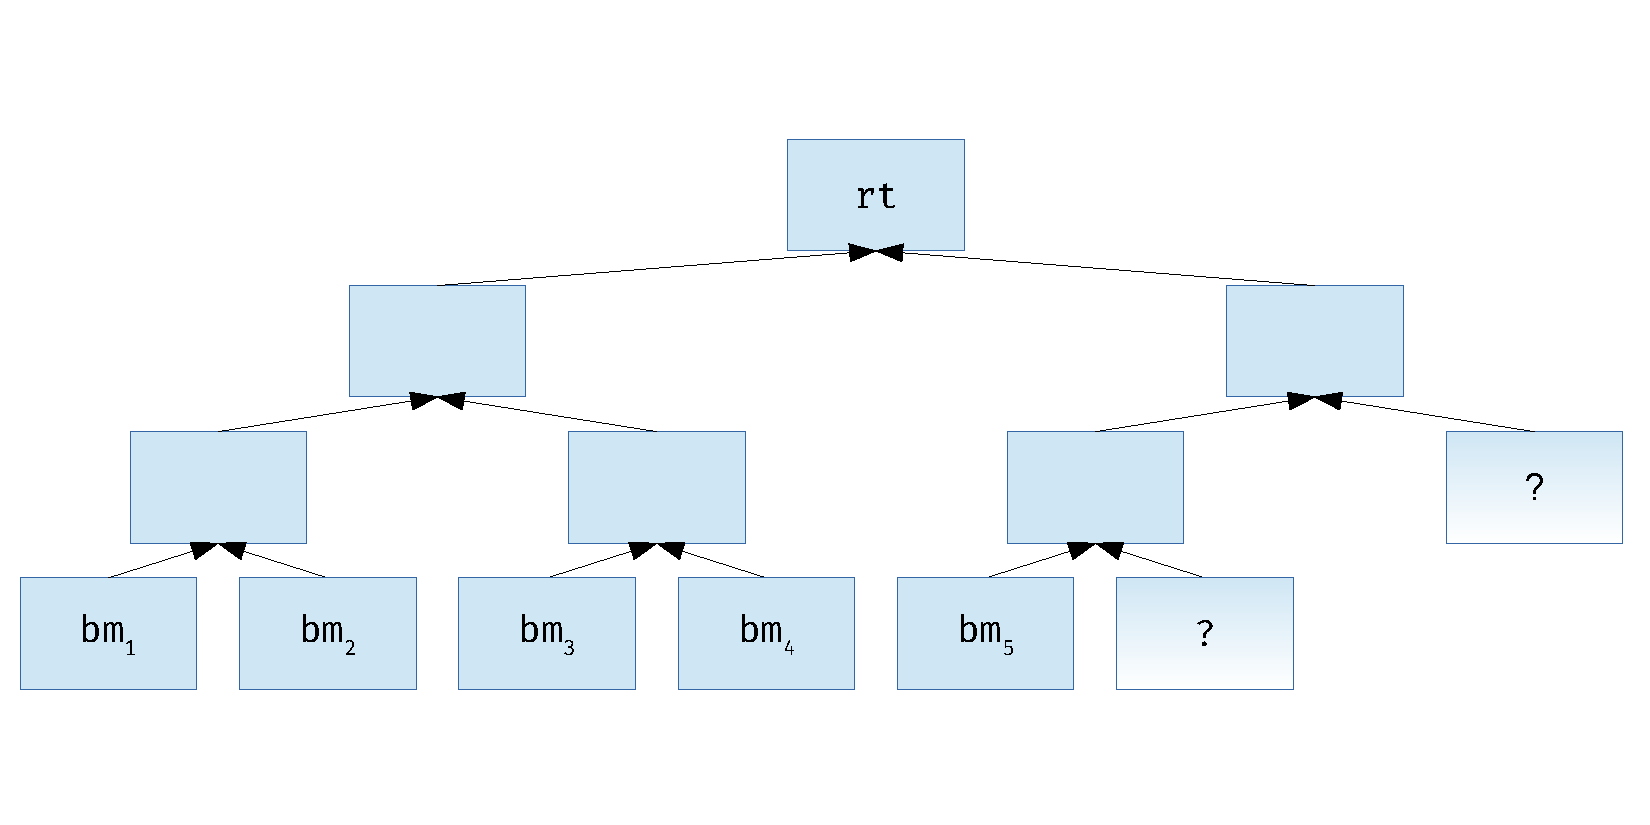
\includegraphics[scale=.4]{incremental_merkle}
\end{center}

\subparagraph{}

The \coinCommitmentTree is an \incrementalMerkleTree of depth $\MerkleDepth$ used to
store \coinCommitments that \PourTransfers produce. Just as the \term{unspent
transaction output set} (UTXO) used in Bitcoin, it is used to express the existence
of value and the capability to spend it. However, unlike the UTXO, it is \emph{not}
the job of this tree to protect against double-spending, as it is append-only.

\subparagraph{}

Blocks in the blockchain are associated (by all nodes) with the root of this tree
after all of its constituent \PourDescriptions' \coinCommitments have been
entered into the tree associated with the previous block.

\subsection{Spent Serials Map}

\subparagraph{}

Transactions insert \serialNumbers into a \spentSerialsMap which is maintained 
alongside the UTXO by all nodes.

\eli{a tx is just a string, so it doesn't insert anything. Rather, nodes process 
tx's and the ``good'' ones lead to the addition of serials to the spent serials 
map.}

Transactions that attempt to insert a \serialNumber into this map that already
exists within it are invalid as they are attempting to double-spend.

\eli{After defining \term{transaction}, one should define what a \term{legal tx} is
(this definition depends on a particular blockchain [view]) and only then can one
talk about ``attempts'' of transactions, and insertions of serial numbers into the
spent serials map.}

\subsection{The Blockchain}

At a given point in time, the \blockchainview of each \fullnode consists of a
sequence of one or more valid \blocks. Each \block consists of a sequence of one or
more \transactions. In a given node's \blockchainview, \treestates are chained in an
obvious way:

\begin{itemize}
  \item The input \treestate of the first \block is the empty \treestate.
  \item The input \treestate of the first \transaction of a \block is the final
        \treestate of the immediately preceding \block.
  \item The input \treestate of each subsequent \transaction in a \block is the
        output \treestate of the immediately preceding \transaction.
  \item The final \treestate of a \block is the output \treestate of its last
        \transaction.
\end{itemize}

An \anchor is a Merkle tree root of a \treestate, and uniquely identifies that
\treestate given the assumed security properties of the Merkle tree's hash function.

Each \transaction is associated with a sequence of \PourDescriptions. TODO They also have
a transparent value flow that interacts with the Pour $\vpubOld$ and $\vpubNew$.
Inputs and outputs are associated with a value.

The total value of the outputs must not exceed the total value of the inputs.

The \anchor of the first \PourDescription in a \transaction must refer to some
earlier \block's final \treestate.

The \anchor of each subsequent \PourDescription may refer either to some earlier
\block's final \treestate, or to the output \treestate of the immediately preceding
\PourDescription.

These conditions act as constraints on the blocks that a \fullnode will
accept into its \blockchainview.

We rely on Bitcoin-style consensus for \fullnodes to eventually converge on their 
views of valid \blocks, and therefore of the sequence of \treestates in those 
\blocks.


\subparagraph{Value pool}

Transaction inputs insert value into a \term{value pool}, and transaction outputs 
remove value from this pool. The remaining value in the pool is available to miners 
as a fee.

\section{Pour Transfers and Descriptions}

A \PourDescription is data included in a \block that describes a \PourTransfer,
i.e. a confidential value transfer. This kind of value transfer is the primary
\Zerocash-specific operation performed by transactions; it uses, but should not be
confused with, the \PourCircuit used for the \zkSNARK proof and verification.

A \PourTransfer spends $\NOld$ \coins $\cOld{1..\NOld}$ and creates $\NNew$ \coins
$\cNew{1..\NNew}$. \Zcash transactions have an additional field $\vpour$, which is a
sequence of \PourDescriptions.

Each \PourDescription consists of:

\begin{list}{}{}

\item $\vpubOldField$ which is a value $\vpubOld$ that the \PourTransfer removes
from the value pool.

\item $\vpubNewField$ which is a value $\vpubNew$ that the \PourTransfer inserts
into the value pool.

\item $\anchorField$ which is a merkle root $\rt$ of the \coinCommitmentTree at
some block height in the past, or the merkle root produced by a previous pour in
this transaction. \sean{We need to be more specific here.}

\item $\scriptSig$ which is a \script that creates conditions for acceptance of a
\PourDescription in a transaction. The $\SHA$ hash of this value is $\hSig$.

\daira{Why $\SHA$ and not $\SHAOrig$? The script is variable-length.}

\item $\scriptPubKey$ which is a \script used to satisfy the conditions of the
$\scriptSig$.

\item $\serials$ which is an $\NOld$ size sequence of serials $\snOld{1..\NOld}$.

\item $\commitments$ which is a $\NNew$ size sequence of \coinCommitments 
$\cmNew{1..\NNew}$.

\item $\TransmitCiphertexts$ which is a $\NNew$ size sequence each element of which
is a \transmittedCiphertext.

\item $\vmacs$ which is a $\NOld$ size sequence of message authentication tags
$\h{1..\NOld}$ that bind $\hSig$ to each $\SpendAuthorityPrivate$ of the
$\PourDescription$.

\item $\zkproof$ which is the zero-knowledge proof $\PourProof$.

\end{list}

\subparagraph{Merkle root validity}

A $\PourDescription$ is valid if $\rt$ is a Coin commitment tree root found in 
either the blockchain or a merkle root produced by inserting the Coin commitments 
of a previous $\PourDescription$ in the transaction to the Coin commitment tree 
identified by that previous $\PourDescription$'s $\anchor$.

\subparagraph{Non-malleability}

A $\PourDescription$ is valid if the script formed by appending $\scriptPubKey$ to 
$\scriptSig$ returns $true$. The $\scriptSig$ is cryptographically bound to 
$\PourProof$.

\subparagraph{Balance}

A \PourTransfer can be seen, from the perspective of the transaction, as an 
input and an output simultaneously. $\vpubOld$ takes value from the value pool and 
$\vpubNew$ adds value to the value pool. As a result, $\vpubOld$ is treated like an 
\emph{output} value, whereas $\vpubNew$ is treated like an \emph{input} value.

\subparagraph{Commitments and Serials}

A \transaction that contains one or more \PourDescriptions, when entered into the 
blockchain, appends to the \coinCommitmentTree with all constituent 
\coinCommitments. All of the constituent \serialNumbers are also entered into the 
\spentSerialsMap of the \blockchainview \emph{and} \mempool. A \transaction is not 
valid if it attempts to add a \serialNumber to the \spentSerialsMap that already 
exists in the map.

\subsection{Pour Circuit and Proofs}

\subparagraph{}

In \Zcash, $\NOld$ and $\NNew$ are both $2$.

\subparagraph{}

A valid instance of $\PourProof$ assures that given a \term{primary input}
$(\rt, \snOld{1..\NOld}, \cmNew{1..\NNew}, \vpubOld, \vpubNew, \hSig, \h{1..\NOld})$,
a witness of \term{auxiliary input}
$(\treepath{1..\NOld}, \cOld{1..\NOld}, \SpendAuthorityPrivateOld{1..\NOld}, \cNew{1..\NNew})$
exists, where:

\begin{list}{}{}

\item for each $i \in \{1..\NOld\}$: $\cOld{i}$ = $(\vOld{i}, 
\SpendAuthorityPublicOld{i}, \CoinCommitRandOld{i}, \CoinAddressRandOld{i})$

\item for each $i \in \{1..\NNew\}$: $\cNew{i}$ = $(\vNew{i}, 
\SpendAuthorityPublicNew{i}, \CoinCommitRandNew{i}, \CoinAddressRandNew{i})$.

\item The following conditions hold:

\end{list}

\subparagraph{Merkle path validity}

for each $i \in \{1..\NOld\}$ $\mid$ $\vOld{i} \neq 0$: $\treepath{i}$ must be a valid path
of depth $\MerkleDepth$ from \linebreak $\CoinCommitment{\cOld{i}}$ to Coin 
commitment merkle tree root $\rt$.

\subparagraph{Balance}

$\vpubOld + \vsum{i=1}{\NOld} \vOld{i} = \vpubNew + \vsum{i=1}{\NNew} \vNew{i}$.

\subparagraph{Serial integrity}

for each $i \in \{1..\NNew\}$: 
$\snOld{i} = \PRFsn{\SpendAuthorityPrivateOld{i}}(\CoinAddressRandOld{i})$.

\subparagraph{Spend authority}

for each $i \in \{1..\NOld\}$:
$\SpendAuthorityPublicOld{i} = \PRFaddr{\SpendAuthorityPrivateOld{i}}(0)$.

\subparagraph{Non-malleability}

% TODO: protocol is really gross here, let's clarify the
% indices and use of PRFpk independence from other h sdfhjgahsdjkgfas
for each $i \in \{1..\NOld\}$: $\h{i}$ = $\PRFpk{\SpendAuthorityPrivateOld{i}}{i}(\hSig)$

\subparagraph{Commitment integrity}

for each $i \in \{1..\NNew\}$: $\cmNew{i}$ = $\CoinCommitment{\cNew{i}}$

\section{Encoding Addresses, Private keys, Coins, and Pour descriptions}

This section describes how \Zcash encodes public addresses, private keys,
coins, and \PourDescriptions.

Addresses, keys, and coins, can be encoded as a byte string; this is called
the \term{raw encoding}. This byte string can then be further encoded using
Base58Check. The Base58Check layer is the same as for upstream \Bitcoin
addresses \cite{Base58Check}.

SHA-256 compression function outputs are always represented as strings of 32
bytes.

The language consisting of the following encoding possibilities is prefix-free.

\subsection{Transparent Public Addresses}

These are encoded in the same way as in \Bitcoin \cite{Base58Check}.

\subsection{Transparent Private Keys}

These are encoded in the same way as in \Bitcoin \cite{Base58Check}.

\subsection{Confidential Public Addresses}

A confidential address consists of $\SpendAuthorityPublic$ and $\TransmitPublic$.
$\SpendAuthorityPublic$ is a SHA-256 compression function output.
$\TransmitPublic$ is an encryption public key (currently ECIES, but this may
change to Curve25519/crypto\_box\_seal), which represents an equivalence class
of two points sharing an $x$ coordinate on an elliptic curve.

\subsubsection{Raw Encoding}

The raw encoding of a confidential address consists of:

\begin{equation*}
\begin{bytefield}[bitwidth=0.07em]{520}
	\bitbox{80}{$\PublicAddressLeadByte$} &
    \bitbox{256}{$\SpendAuthorityPublic$ (32 bytes)} &
    \bitbox{256}{A 33-byte encoding of $\TransmitPublic$}
\end{bytefield}
\end{equation*}

\begin{itemize}
    \item A byte, $\PublicAddressLeadByte$, indicating this version of the
        raw encoding of a \Zcash public address.
    \item 32 bytes specifying $\SpendAuthorityPublic$.
    \item An encoding of $\TransmitPublic$: The byte $\mathbf{0x01}$, followed by 32 bytes
        representing the $x$ coordinate of an elliptic curve point according to
        the $\mathsf{FE2OSP}$ primitive specified in section 5.5.4 of IEEE Std 1363-2000.
        [Non-normative note: Since the curve is over a prime field, this is just
            the 32-byte big-endian representation of the $x$ coordinate. The
            overall encoding matches the $\mathsf{EC2OSP{\mhyphen}X}$ primitive
            specified in section 5.5.6.3 of IEEE Std 1363a-2004. It does not
            matter which of the two points with the same $x$ coordinate is used.]
\end{itemize}

\daira{check that this lead byte is distinct from other Bitcoin stuff,
and produces `z' as the Base58Check leading character.}

\nathan{what about the network version byte?}

\daira{add bibliographic references for the IEEE standards.}

\subsection{Confidential Address Secrets}

A confidential address secret consists of $\SpendAuthorityPrivate$ and
$\TransmitPrivate$. $\SpendAuthorityPrivate$ is a SHA-256 compression function
output. $\TransmitPrivate$ is an encryption private key (currently ECIES), which
is an integer.

\subsubsection{Raw Encoding}

The raw encoding of a confidential address secret consists of, in order:

\begin{equation*}
\begin{bytefield}[bitwidth=0.07em]{520}
	\bitbox{80}{$\PrivateAddressLeadByte$} &
    \bitbox{256}{$\SpendAuthorityPrivate$ (32 bytes)} &
    \bitbox{256}{$\TransmitPrivate$ (32 bytes)}
\end{bytefield}
\end{equation*}

\begin{itemize}
    \item A byte $\PrivateAddressLeadByte$ indicating this version of the
        raw encoding of a \Zcash private key.
    \item 32 bytes specifying $\SpendAuthorityPrivate$.
    \item 32 bytes specifying a big-endian encoding of $\TransmitPrivate$.
\end{itemize}

\daira{check that this lead byte is distinct from other Bitcoin stuff,
and produces `z' as the Base58Check leading character.}

\nathan{what about the network version byte?}

\subsection{Coins}

Transmitted coins are stored on the blockchain in encrypted form, together with
a \coinCommitment $\cm$.

A \transmittedCiphertext is an ECIES encryption of a \transmittedPlaintext to a
\transmitPublicAlgorithm key $\TransmitPublic$.

A \transmittedPlaintext consists of $(\Value, \CoinAddressRand, \CoinCommitRand)$,
where:

\begin{itemize}
    \item $\Value$ is a 64-bit unsigned integer representing the value of the
        \coin in \zatoshi (1 \ZEC = $10^8$ \zatoshi).
    \item $\CoinAddressRand$ is a 32-byte $\PRFsn{\SpendAuthorityPrivate}$ seed.
    \item $\CoinCommitRand$ is a 32-byte \COMMtrapdoor.
\end{itemize}

Note that the value $\mathsf{s}$ described as being part of a coin in the \Zerocash
paper is not encoded because it is fixed to zero.

\subsection{Raw Encoding}

The raw encoding of a \transmittedPlaintext consists of, in order:

\begin{equation*}
\begin{bytefield}[bitwidth=0.05em]{200}
	\bitbox{80}{$\TransmitPlaintextVersionByte$} &
    \bitbox{230}{$\Value$ (8 bytes, big endian)} &
    \bitbox{230}{$\CoinAddressRand$ (32 bytes)} &
    \bitbox{230}{$\CoinCommitRand$ (32 bytes)} &
\end{bytefield}
\end{equation*}

\begin{itemize}
    \item A byte $\TransmitPlaintextVersionByte$ indicating this version of the raw 
encoding of a \transmittedPlaintext.
    \item 8 bytes specifying a big-endian encoding of $\Value$.
    \item 32 bytes specifying $\CoinAddressRand$.
    \item 32 bytes specifying $\CoinCommitRand$.
\end{itemize}

\section{Pours (within a transaction on the blockchain)}

TBD.

\section{Transactions}

TBD.

\section{References}

\begingroup
\renewcommand{\section}[2]{}
\bibliographystyle{plain}
\bibliography{zcash}
\endgroup

\end{document}
